% Source: physical PDF p. 139 (printed p. 116). Coverage: Figure 18.2 and complete caption. Uncertainty: none; vector geometry reconstructed from the rendered scan.
\begin{figure}[htbp]
 \centering
 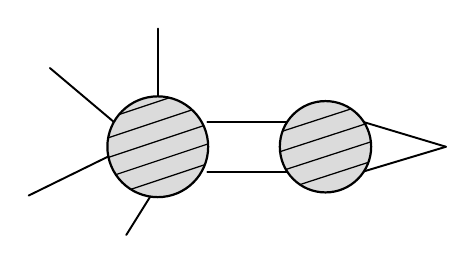
\begin{tikzpicture}[x=1cm,y=1cm,line cap=round,line join=round]
  \draw[line width=0.7pt] (-2.55,1.00) -- (-1.72,0.30);
  \draw[line width=0.7pt] (-2.82,-0.62) -- (-1.76,-0.10);
  \draw[line width=0.7pt] (-1.58,-1.12) -- (-1.23,-0.56);
  \draw[line width=0.7pt] (-1.18,1.50) -- (-1.18,0.62);
  \draw[line width=0.7pt] (-0.55,0.32) -- (0.70,0.32);
  \draw[line width=0.7pt] (-0.55,-0.32) -- (0.70,-0.32);
  \draw[line width=0.7pt] (1.28,0.36) -- (2.48,0);
  \draw[line width=0.7pt] (1.28,-0.36) -- (2.48,0);
  \fill[gray!28] (-1.18,0) circle[radius=0.64];
  \fill[gray!28] (0.95,0) circle[radius=0.58];
  \begin{scope}
   \clip (-1.18,0) circle[radius=0.64];
   \foreach \a in {-1.25,-1.00,...,1.25}
    \draw[line width=0.45pt] (-2.15,\a) -- (-0.20,{\a+0.65});
  \end{scope}
  \begin{scope}
   \clip (0.95,0) circle[radius=0.58];
   \foreach \a in {-1.20,-0.95,...,1.20}
    \draw[line width=0.45pt] (-0.05,\a) -- (1.95,{\a+0.65});
  \end{scope}
  \draw[line width=0.8pt] (-1.18,0) circle[radius=0.64];
  \draw[line width=0.8pt] (0.95,0) circle[radius=0.58];
 \end{tikzpicture}
 \renewcommand{\thefigure}{18.2}
 \caption{A class of Feynman diagrams for the matrix element of the operator $\int d^4x\,\exp(-ip\cdot x)\,\phi^2(x)$ that exhibit an ultraviolet divergence. The notation is the same as in Figure~\ref{fig:18.1}.}
 \label{fig:18.2}
\end{figure}
